\chapter{Practical Results}
\label{chp:prac_results}
%WHAT you are going to present in this chapter/section
%WHY you are presenting it, and
%HOW you are going to present it






\section{Swingup Controller}
%WHAT you are going to present in this chapter/section
%WHY you are presenting it, and
%HOW you are going to present it
This section provides the practical results of the swing-up controller and discusses the differences it contains with the simulation. \\

\begin{figure}[h]
	\centering
	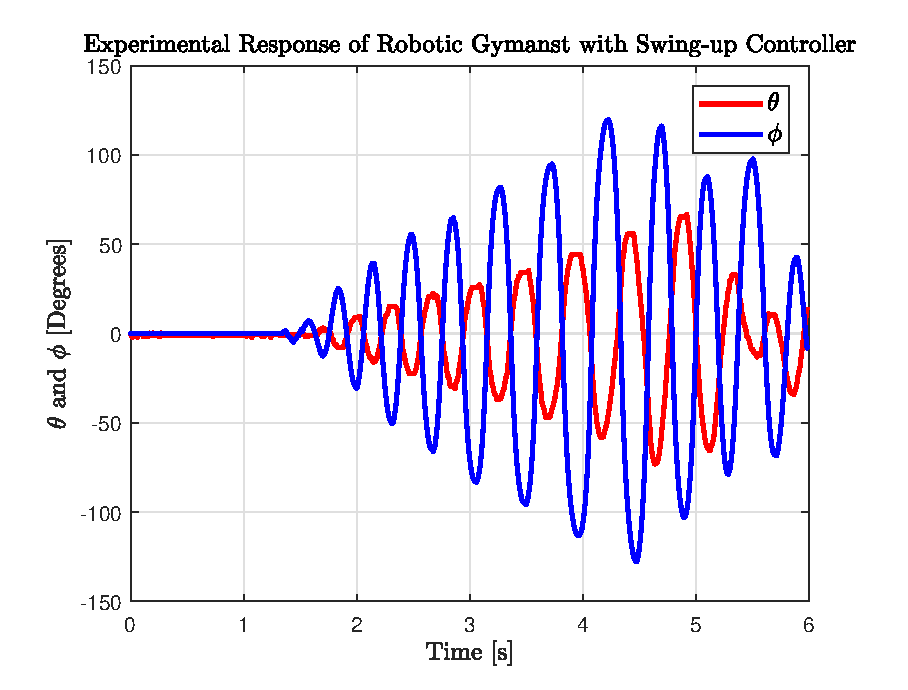
\includegraphics[scale=1]{./figs/experiment_swingup.eps}
	\caption{Experimental Response of the Robotic Gymnast with Swing-up Controller}
	\label{fig:experiment_swingup}
\end{figure}


Figure \ref{fig:experiment_swingup} shows the practical results of the swing-up controller and contains interesting behaviour that the simulation does not contain. The swing-up controller did not require a initial condition as in the simulation. The system started to swing-up from the rest position because of the noise being introduced by the ADC. This noise is amplified by using the numerical differential algorithm to calculate the angular velocity of the pendulums that is required by the swing-up controller. The swing-up controller reacts on this small error which results in the motor to output a torque and provides this small initial condition.\\




\section{Balancing Controller}
%WHAT you are going to present in this chapter/section
%WHY you are presenting it, and
%HOW you are going to present it
\section{Swingup and Balancing}
%WHAT you are going to present in this chapter/section
%WHY you are presenting it, and
%HOW you are going to present it